% $Header: /Users/joseph/Documents/LaTeX/beamer/solutions/conference-talks/conference-ornate-20min.en.tex,v 90e850259b8b 2007/01/28 20:48:30 tantau $

\documentclass{beamer}

% This file is a solution template for:

% - Talk at a conference/colloquium.
% - Talk length is about 20min.
% - Style is ornate.



% Copyright 2004 by Till Tantau <tantau@users.sourceforge.net>.
%
% In principle, this file can be redistributed and/or modified under
% the terms of the GNU Public License, version 2.
%
% However, this file is supposed to be a template to be modified
% for your own needs. For this reason, if you use this file as a
% template and not specifically distribute it as part of a another
% package/program, I grant the extra permission to freely copy and
% modify this file as you see fit and even to delete this copyright
% notice. 


\mode<presentation>
{
  \usetheme{CambridgeUS}
  % or ...

  \setbeamercovered{transparent}
  % or whatever (possibly just delete it)
  
\makeatletter
\setbeamertemplate{headline}{%
\leavevmode%
  \hbox{%
    \begin{beamercolorbox}[wd=.5\paperwidth,ht=2.25ex,dp=1ex]{section in head/foot}%
    \usebeamerfont{section in head/foot}\,\insertsection
    \end{beamercolorbox}%
    \begin{beamercolorbox}[wd=.5\paperwidth,ht=2.25ex,dp=1ex,right]{subsection in head/foot}%
    \usebeamerfont{section in head/foot}The ALICE Collaboration\,
    \end{beamercolorbox}%
  }
}
\makeatother
}

\usepackage[english]{babel}
% or whatever

\usepackage[latin1]{inputenc}
% or whatever

\usepackage{times}
\usepackage[T1]{fontenc}
% Or whatever. Note that the encoding and the font should match. If T1
% does not look nice, try deleting the line with the fontenc.
%particles
\newcommand{\jpsi}{\rm J/$\psi$}
\newcommand{\psip}{$\psi^\prime$}
\newcommand{\jpsiDY}{\rm J/$\psi$\,/\,DY}
\newcommand{\chic}{$\chi_{\rm c}$}
\newcommand{\pip}{$\pi^{+}$}
\newcommand{\pim}{$\pi^{-}$}
\newcommand{\pizero}{$\pi^{0}$}
\newcommand{\kap}{K$^{+}$}
\newcommand{\kam}{K$^{-}$}
\newcommand{\pbar}{$\rm\overline{p}$}
\newcommand{\ccbar}{\ensuremath{\mathrm{c\overline{c}}}}
\newcommand{\bbbar}{\ensuremath{\mathrm{b\overline{b}}}}
\newcommand{\Dzero}{\ensuremath{\mathrm{D^{0}}}}
\newcommand{\Dzerobar}{\ensuremath{\mathrm{\overline{D}^{0}}}}
\newcommand{\Dpm}{\ensuremath{\mathrm{D^{\pm}}}}
\newcommand{\Ds}{\ensuremath{\mathrm{D_{s}^{\pm}}}}
\newcommand{\Dstar}{\ensuremath{\mathrm{D^{*\pm}}}}

%collision systems
\newcommand{\pp}{pp}
\newcommand{\pPb}{p--Pb}
\newcommand{\PbPb}{Pb--Pb}

%detectors
\newcommand{\ezdc}{$E_{\rm ZDC}$}

%units
\newcommand{\GeVc}{GeV/$c$}
\newcommand{\GeVcsq}{GeV/$c^2$}

%others
\newcommand{\degree}{$^{\rm o}$}
\newcommand{\s}{\ensuremath{\sqrt{s}}}
\newcommand{\snn}{\ensuremath{\sqrt{s_{\rm NN}}}}
\newcommand{\y}{\ensuremath{y}}
\newcommand{\pt}{\ensuremath{p_{\rm T}}}
\newcommand{\dedx}{d$E$/d$x$}
\newcommand{\dndy}{d$N$/d$y$}
\newcommand{\dndydpt}{${\rm d}^2N/({\rm d}y {\rm d}p_{\rm t})$}
\newcommand{\zpar}{\ensuremath{z_{||}}}
\newcommand{\zpargen}{\ensuremath{z_{||}^{\mathrm{part}}}}
\newcommand{\zpardet}{\ensuremath{z_{||}^{\mathrm{det}}}}
\newcommand{\ptchjet}{\ensuremath{p_{\mathrm{T,ch\, jet}}}}
\newcommand{\ptjet}{\ensuremath{p_{\mathrm{T,jet}}}}
\newcommand{\ptchjetgen}{\ensuremath{p_{\mathrm{T,ch\,jet}}^{\mathrm{part}}}}
\newcommand{\ptchjetdet}{\ensuremath{p_{\mathrm{T,ch\,jet}}^{\mathrm{det}}}}
\newcommand{\ptd}{\ensuremath{p_{\mathrm{T,D}}}}
\newcommand{\ptdgen}{\ensuremath{p_{\mathrm{T,D}}^{\mathrm{part}}}}
\newcommand{\ptddet}{\ensuremath{p_{\mathrm{T,D}}^{\mathrm{det}}}}
\newcommand{\antikt}{anti-\ensuremath{k_{\mathrm{T}}}}
\newcommand{\Antikt}{Anti-\ensuremath{k_{\mathrm{T}}}}
\newcommand{\kt}{\ensuremath{k_{\mathrm{T}}}}
\newcommand{\pthard}{\ensuremath{p_{\mathrm{T,hard}}}}

\title[D-tagged jets in pp collisions at 7 TeV] % (optional, use only with long paper titles)
{D-meson tagged jets in pp collisions at 7 TeV}

\author[Salvatore Aiola]% (optional, use only with lots of authors)
{Salvatore Aiola (Yale University),\\
on behalf of the ALICE Collaboration\\
\bigskip

\includegraphics[height=2cm]{img/yale}\quad

\includegraphics[height=2cm]{img/alice}}
% - Give the names in the same order as the appear in the paper.
% - Use the \inst{?} command only if the authors have different
%   affiliation.

\institute[Yale University] % (optional, but mostly needed)


\date[Hot Quarks 2016] % (optional, should be abbreviation of conference name)
{Hot Quarks 2016, September 12-17, South Padre Island, TX}
% - Either use conference name or its abbreviation.
% - Not really informative to the audience, more for people (including
%   yourself) who are reading the slides online

\subject{High-Energy Physics}
% This is only inserted into the PDF information catalog. Can be left
% out. 



% If you have a file called "university-logo-filename.xxx", where xxx
% is a graphic format that can be processed by latex or pdflatex,
% resp., then you can add a logo as follows:

% \pgfdeclareimage[height=0.5cm]{university-logo}{university-logo-filename}
% \logo{\pgfuseimage{university-logo}}


% If you wish to uncover everything in a step-wise fashion, uncomment
% the following command: 

%\beamerdefaultoverlayspecification{<+->}


\begin{document}

\begin{frame}
  \titlepage
\end{frame}

\begin{frame}{Outline}
  \tableofcontents
  % You might wish to add the option [pausesections]
\end{frame}


% Structuring a talk is a difficult task and the following structure
% may not be suitable. Here are some rules that apply for this
% solution: 

% - Exactly two or three sections (other than the summary).
% - At *most* three subsections per section.
% - Talk about 30s to 2min per frame. So there should be between about
%   15 and 30 frames, all told.

% - A conference audience is likely to know very little of what you
%   are going to talk about. So *simplify*!
% - In a 20min talk, getting the main ideas across is hard
%   enough. Leave out details, even if it means being less precise than
%   you think necessary.
% - If you omit details that are vital to the proof/implementation,
%   just say so once. Everybody will be happy with that.

\section{Physics Motivations}

\subsection{Charm and pQCD}
\begin{frame}{D-Meson Cross Sections}
\begin{columns}
\column{.5\textwidth}
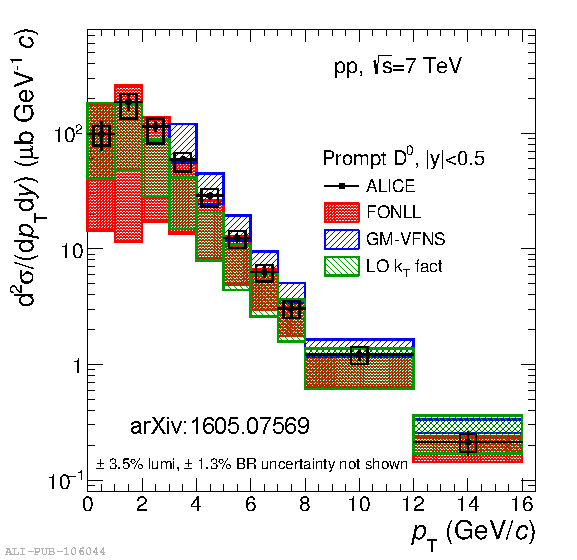
\includegraphics[width=\textwidth]{img/ALICE_D0Meson}

\column{.5\textwidth}
\textbf{\alert{Sensitive test of pQCD}}
\begin{itemize}
\item D mesons measured down to \alert{$\ptd=0$~\GeVc}
\item \alert{$m_{\rm c} \neq 0$}~$\rightarrow$ pQCD is applicable
\item large theoretical uncertainties at low \ptd $\rightarrow$ \alert{small $x$, $Q^2$}
\begin{itemize}
\item renormalization scale
\item gluon PDFs
\end{itemize}
\end{itemize}
\end{columns}
\end{frame}

\begin{frame}{D-Tagged Jets}
\begin{columns}
\column{.5\textwidth}
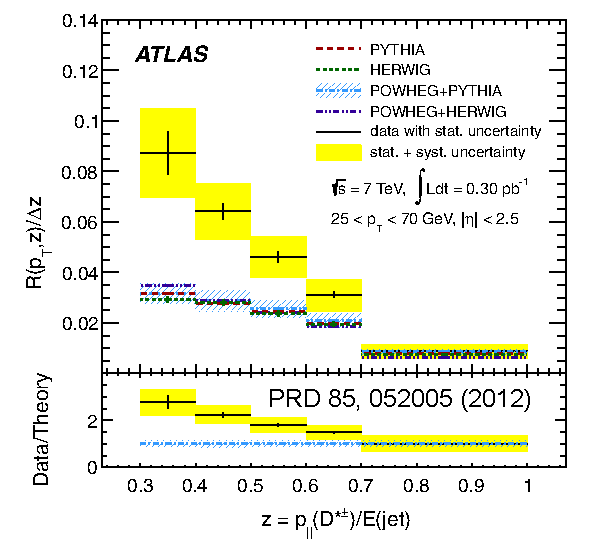
\includegraphics[width=\textwidth]{img/ATLAS_DStarJets}

\column{.5\textwidth}
\begin{itemize}
\item \alert{Few measurements} of D-tagged jets have been published
\item \alert{Large discrepancy} with pQCD-based Monte Carlo generators
\item D-tagged jets can help to pin-point weaknesses in our understanding of QCD
\begin{itemize}
\item charm production mechanism?
\item fragmentation functions?
\end{itemize}
\end{itemize}
\end{columns}
\end{frame}

\subsection{Charm and the QGP}
\begin{frame}{Probe of the Quark-Gluon Plasma}
\begin{columns}
\column{.5\textwidth}
\textbf{\alert{Self-produced probe}}
\begin{itemize}
\item c quarks are \alert{produced early} in the collision
\item Interact with the medium
\begin{columns}
\column{.4\textwidth}
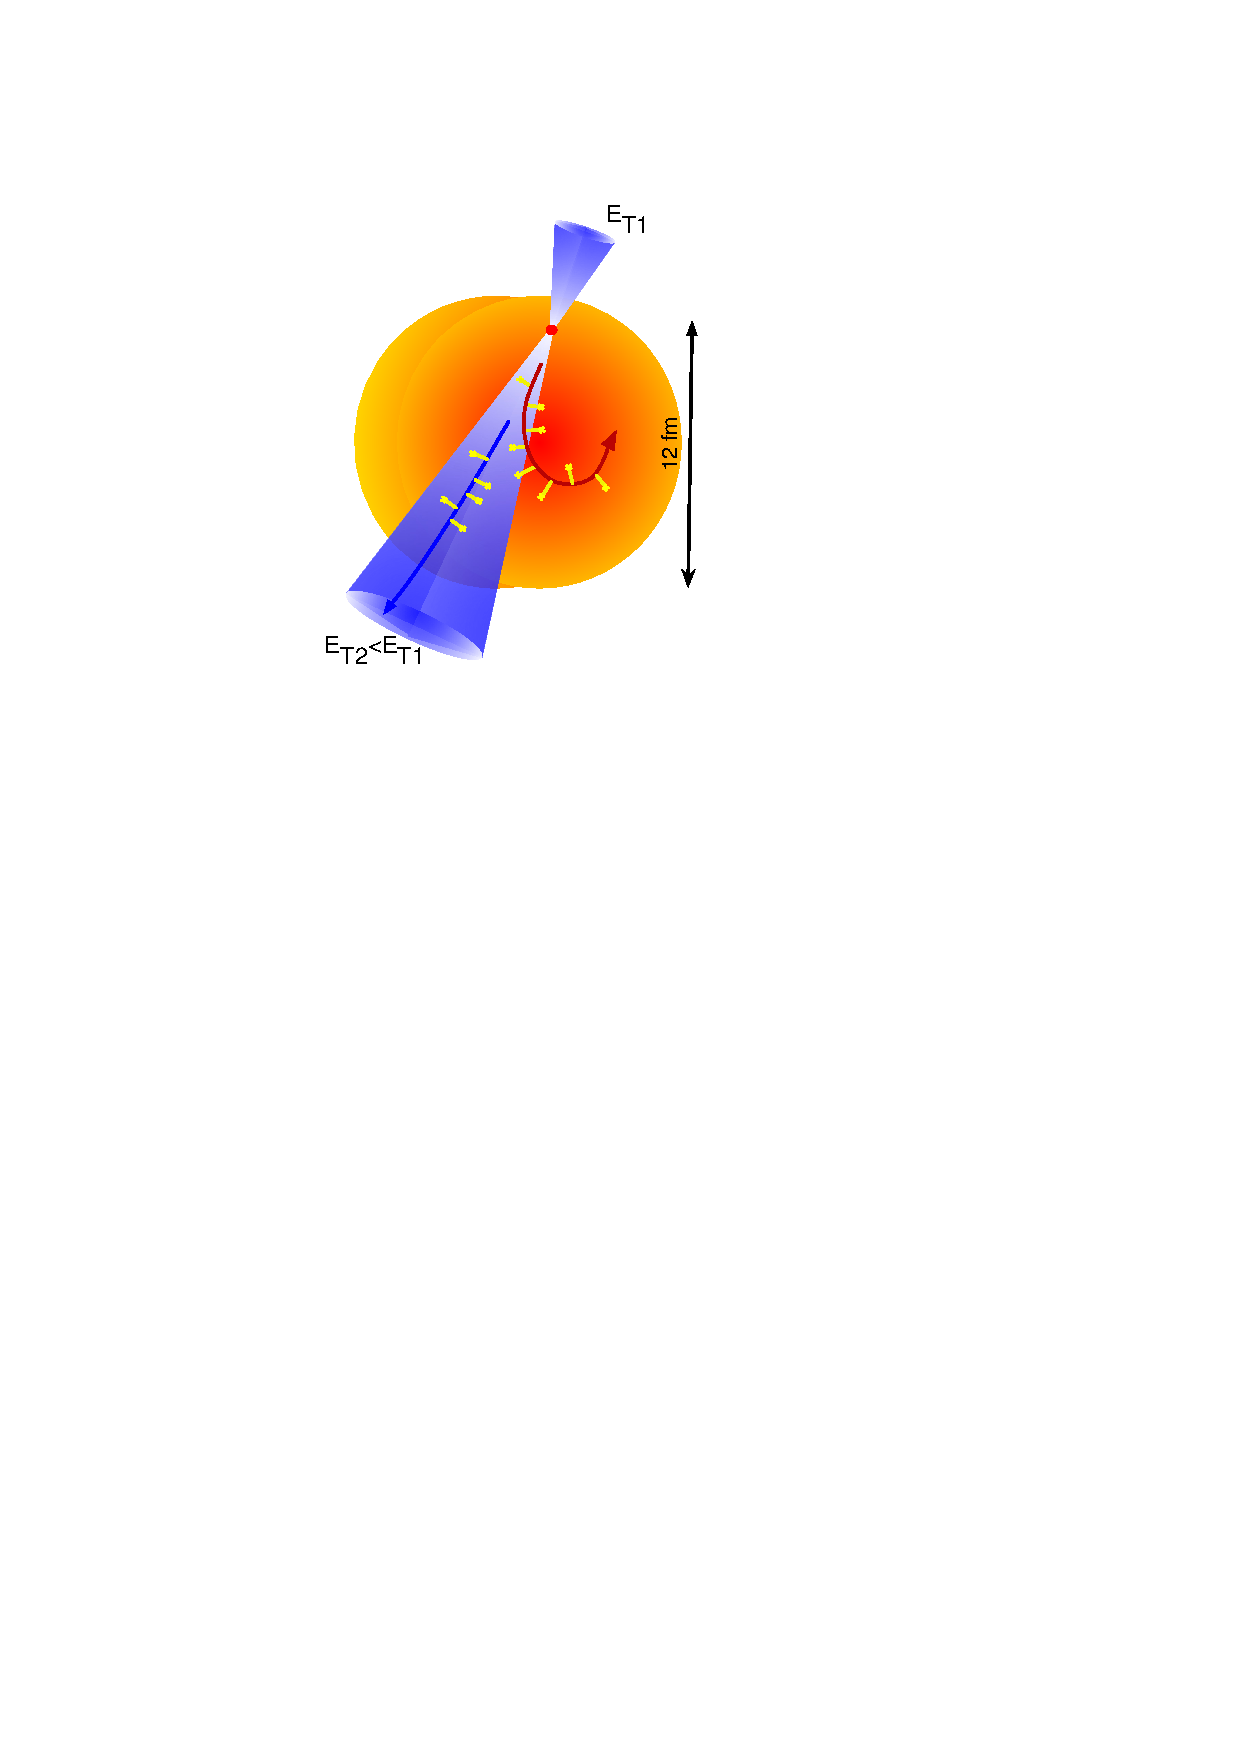
\includegraphics[width=\textwidth]{img/jetquenching}
\column{.6\textwidth}
\begin{itemize}
\item collisional energy loss
\item radiative energy loss (\alert{dead-cone effect})
\end{itemize}
\end{columns}
\item Hint of slightly \alert{smaller suppression} compared to pions at low \pt
\end{itemize}

\column{.5\textwidth}
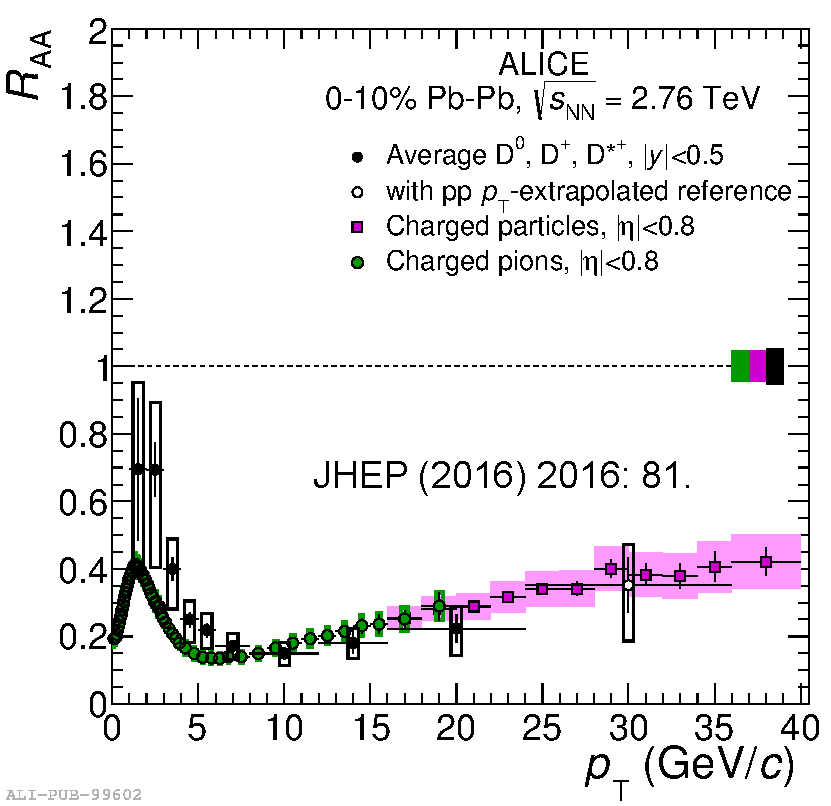
\includegraphics[width=\textwidth]{img/ALICE_DMesonRAA}
\end{columns}
\end{frame}

\section{Analysis Overview}

\subsection{ALICE at the LHC}
\begin{frame}{ALICE at the LHC}
\begin{columns}

\column{.55\textwidth}
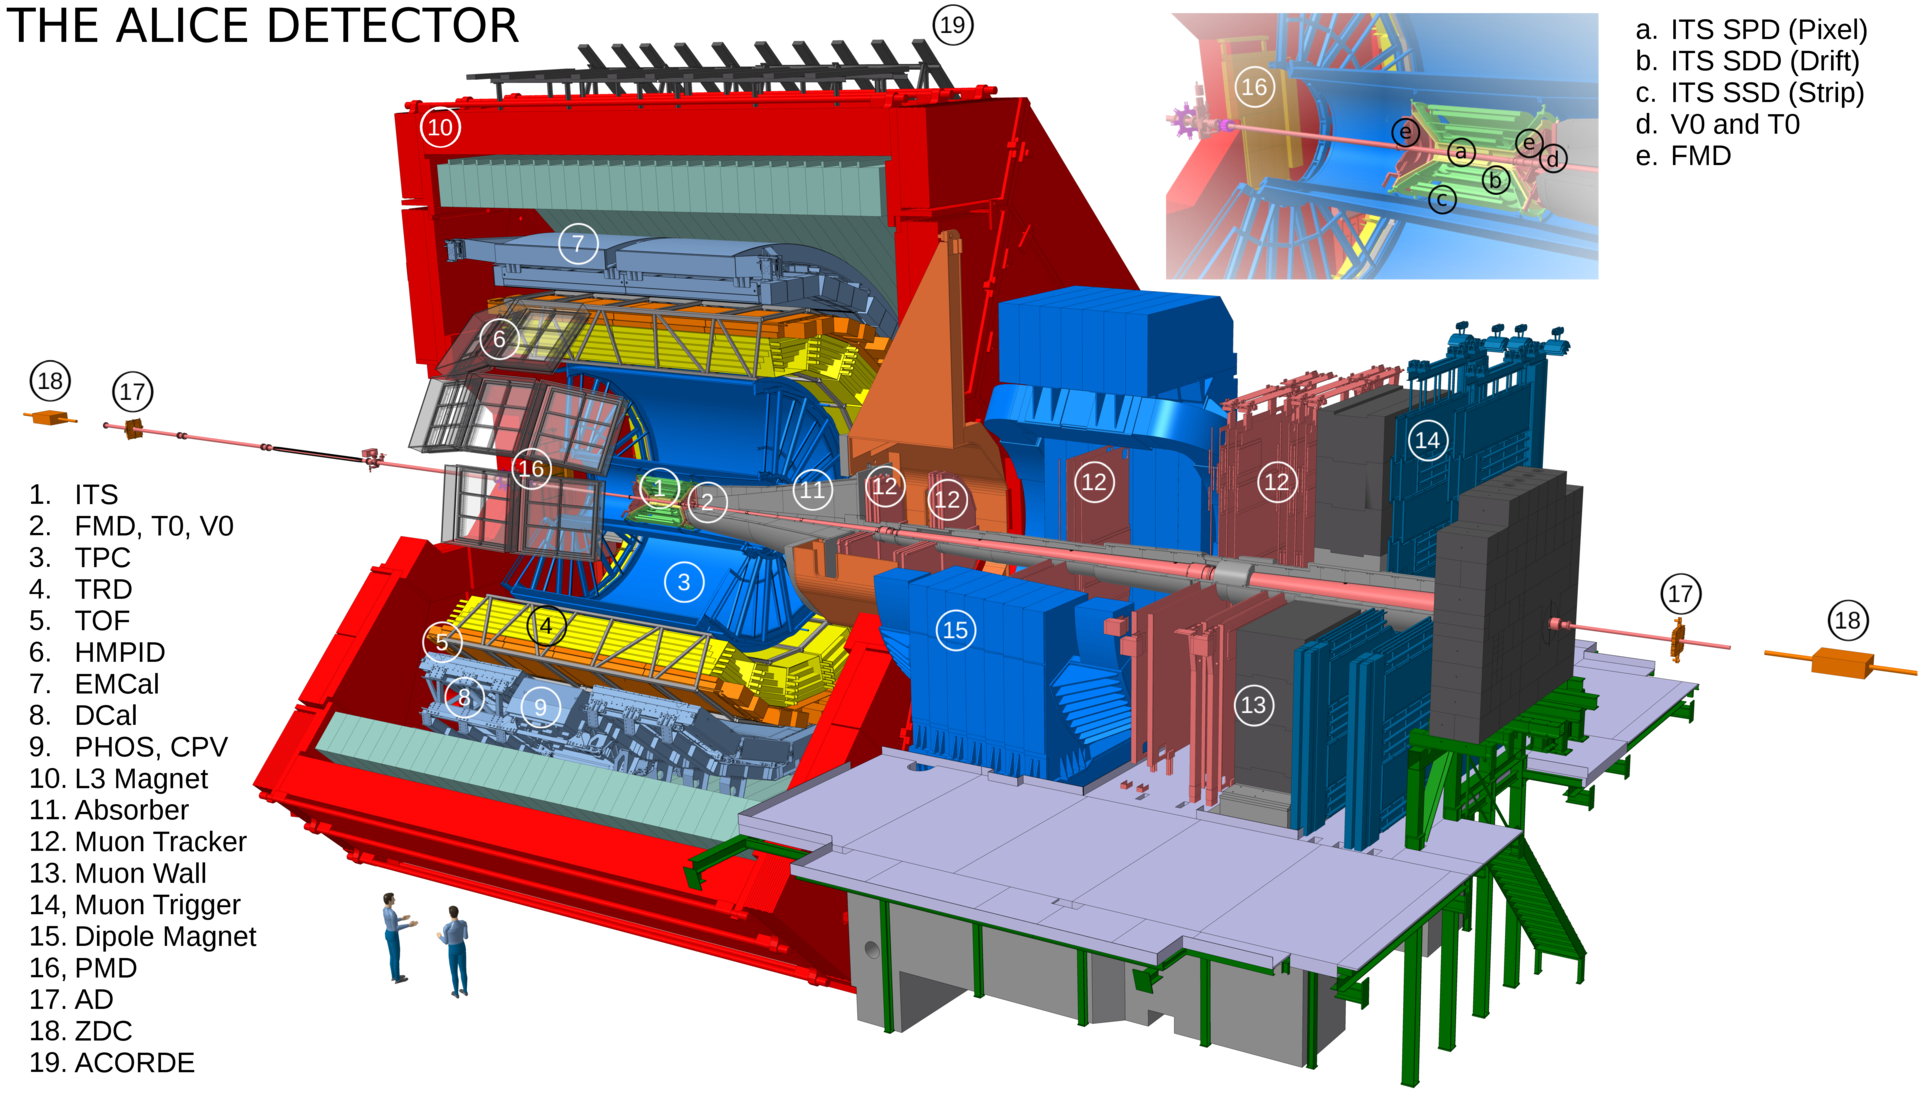
\includegraphics[width=\textwidth]{img/ALICE_Schematics}

\column{.45\textwidth}
\begin{itemize}
\item Strongest points
\begin{itemize}
\item \alert{PID} (e, $\gamma$, $\pi$, K, p, d, ${}^3$He)
\item \alert{low-momentum tracking} ($\pt > 0.15$~\GeVc)
\end{itemize}
\item \alert{D mesons} via hadronic decays (TPC, ITS, TOF)
\begin{itemize}
\item PID, topological cuts
\item invariant mass analysis
\end{itemize}
\item \alert{Jet reconstruction} using \antikt\ algorithm
\begin{itemize}
\item charged constituents (TPC, ITS)
\item neutral constituents (EMCal, DCal)
\end{itemize}
\end{itemize}
\end{columns}
\end{frame}

\subsection{D-meson jet tagging}
\begin{frame}{D-meson jet tagging}

\begin{columns}

\column{0.6\textwidth}
\begin{enumerate}
\item \Dzero\ meson candidates are identified through \alert{PID} and \alert{topological} cuts
\item For each \Dzero\ candidate run the \alert{jet finding} among all other reconstructed tracks
\item Combinatorial background from random $\mathrm{K}\pi$ pairs subtracted on a ensemble basis via an \alert{invariant mass analysis}
\end{enumerate}

\column{0.4\textwidth}
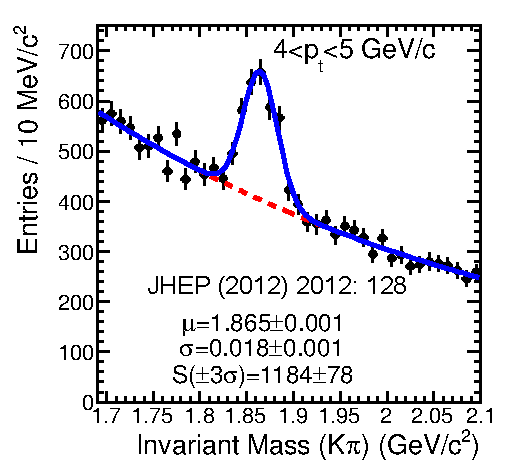
\includegraphics[width=\textwidth]{img/ALICE_D0InvMass}
\end{columns}
\bigskip
\textbf{\alert{\Dzero(\Dzerobar) meson}}
\begin{itemize}
\item $M=1.865$~\GeVcsq, $c\tau=312\,\mu\mathrm{m}$ 
\item Decay: \Dzero$\rightarrow\mathrm{K}^+\pi^-$ and c.c.
\end{itemize}

\end{frame}

\section{Detector Perfomance}

\subsection{D-tagged jet reconstruction efficiency}
\begin{frame}{D-tagged jet reconstruction efficiency}

\begin{columns}
\column{.6\textwidth}
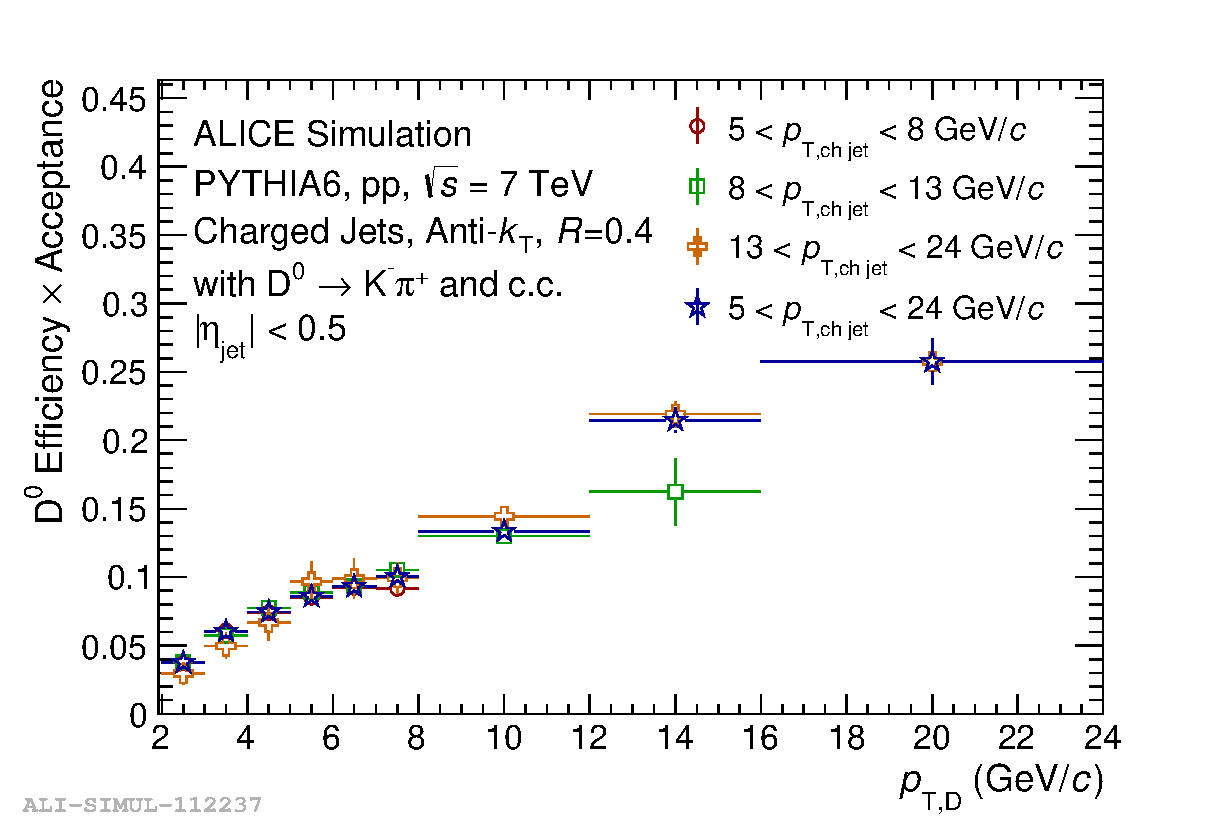
\includegraphics[width=\textwidth]{img/HQ16_Simulation_EfficiencyVsDPt}
\column{.4\textwidth}
Monte Carlo simulation
\begin{itemize}
\item PYTHIA6 Perugia-2011
\item GEANT3: detailed description of ALICE
\end{itemize}
\bigskip
\alert{Steep dependence on the \ptd}
\begin{itemize}
\item[$\rightarrow$] topological cuts on the secondary vertex, tighter at low \ptd\
\end{itemize}
\end{columns}
\bigskip
\alert{No dependence on the \ptchjet}: simplifies corrections and reduces systematic uncertainties 
\end{frame}

\subsection{JES shift and \pt\ resolution}
\begin{frame}{JES shift and \pt\ resolution}

\begin{columns}
\column{.32\textwidth}
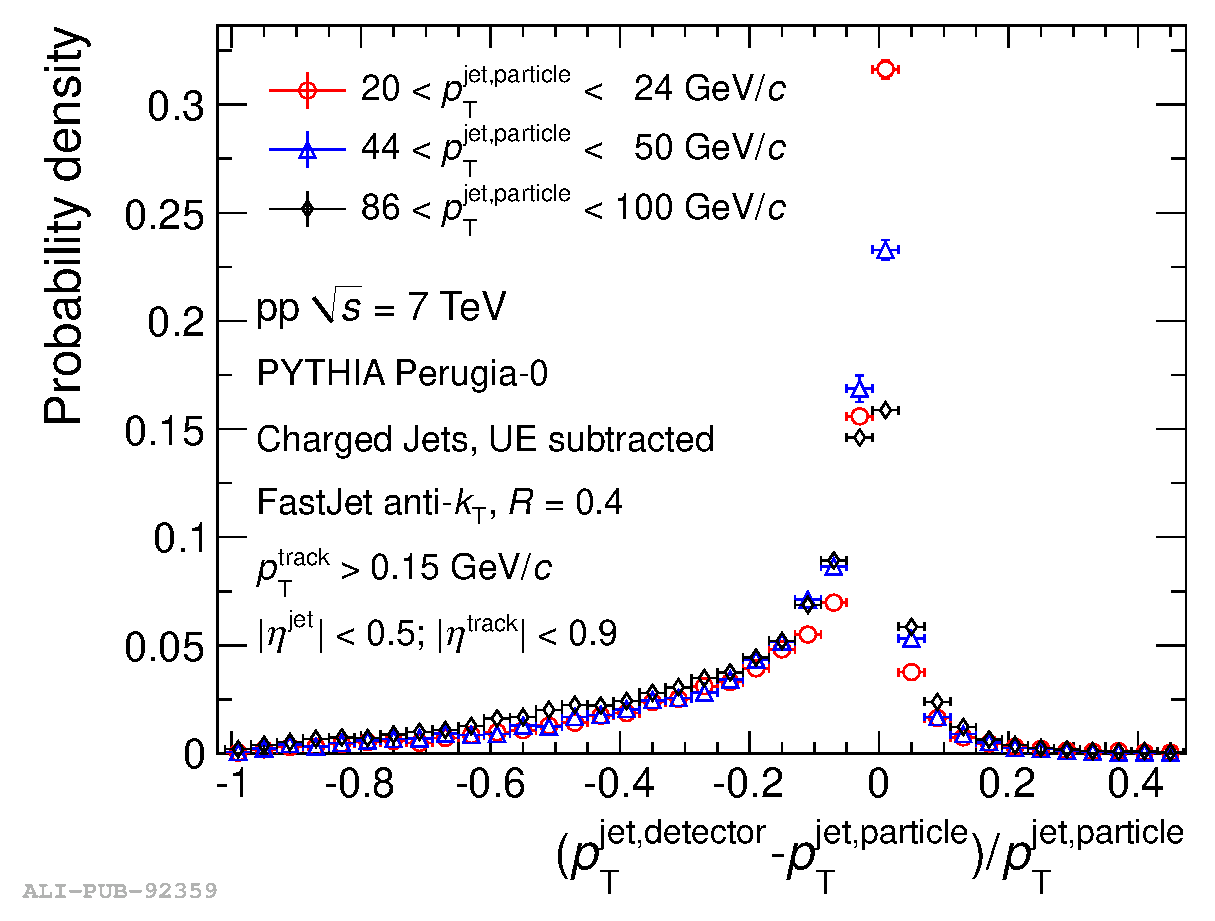
\includegraphics[width=\textwidth]{img/ALICE_JetRes}
\column{.32\textwidth}
\centering
\textcolor{red}{$\leftarrow$Inclusive Jets: $\mu\approx -3\%$, \textbf{$\sigma\approx17\%$}}
\textcolor{blue}{D-Tagged Jets: $\mu\approx -3\%$, \textbf{$\sigma\approx11\%$ }$\rightarrow$}
slightly better \pt\ resolution due to the D-meson requirement
\column{.36\textwidth}
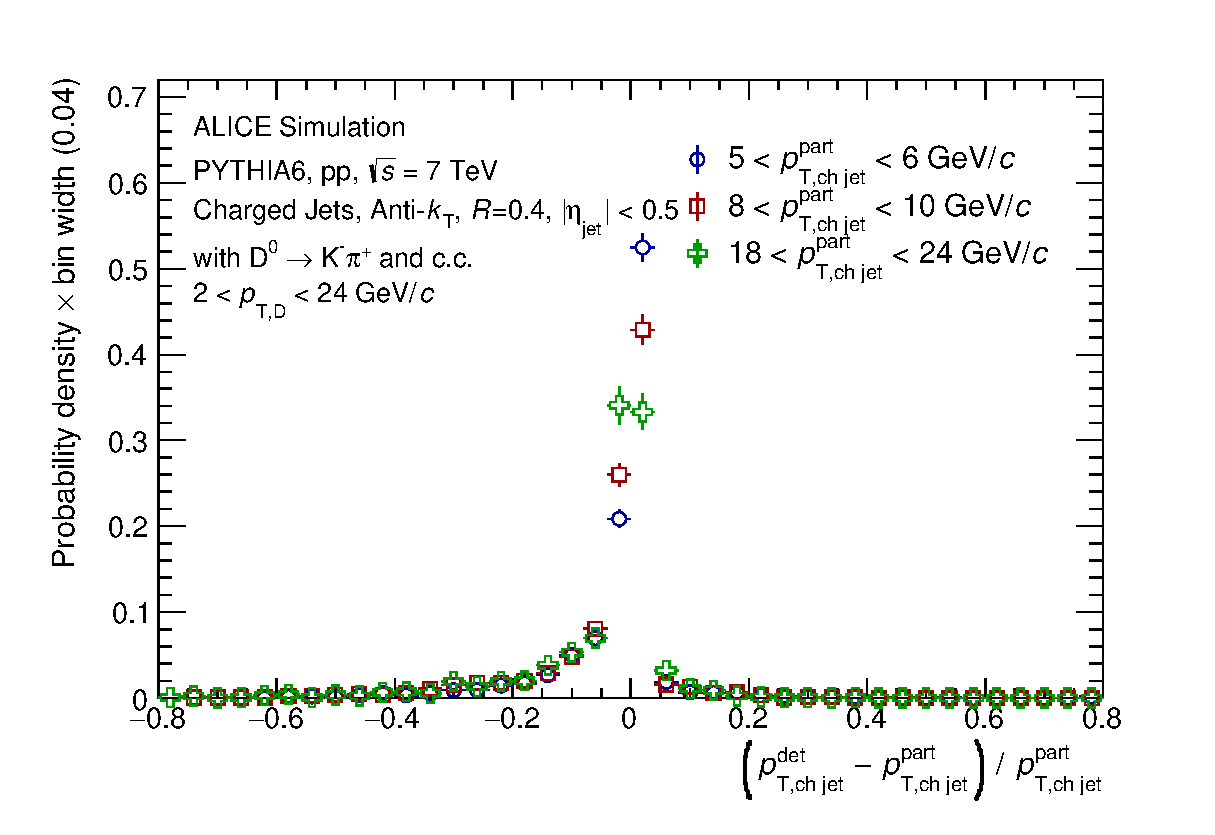
\includegraphics[width=\textwidth]{img/HQ16_Simulation_DetectorResponse}
\end{columns}
\smallskip
\centering
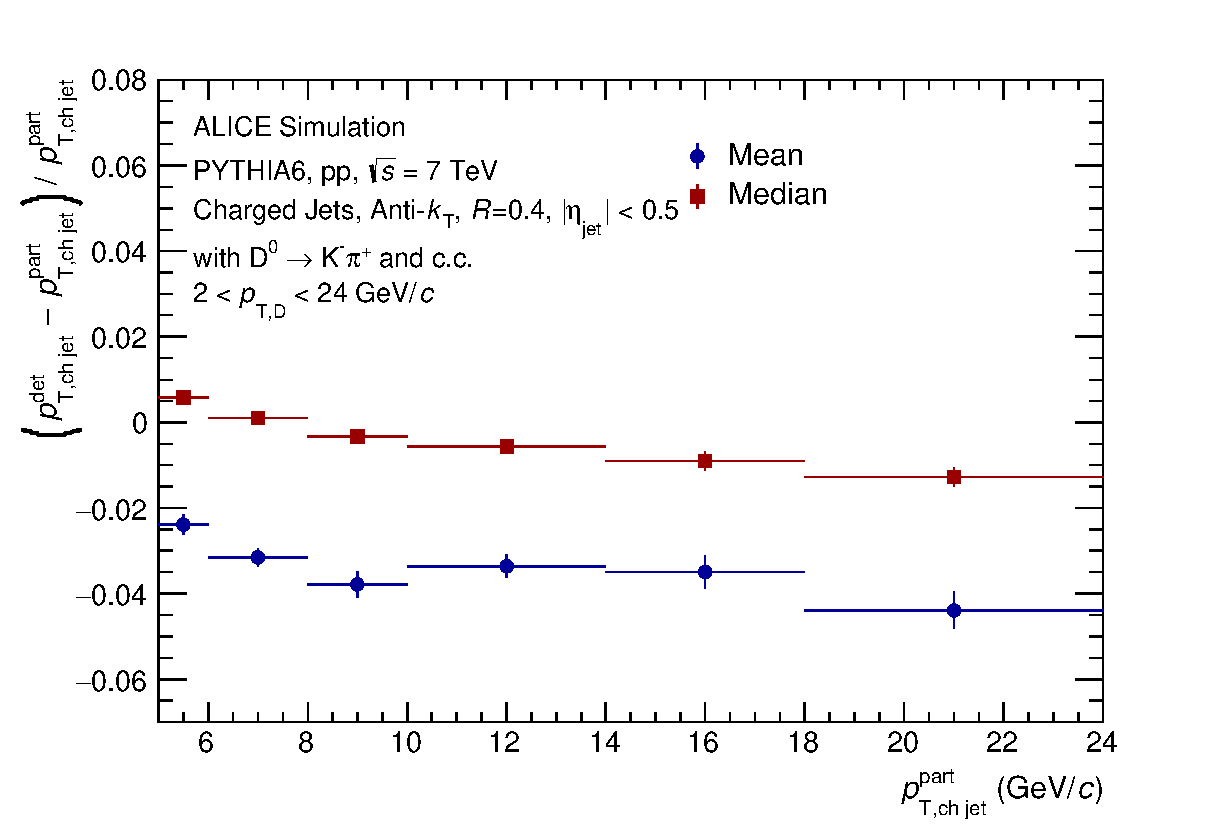
\includegraphics[width=.36\textwidth]{img/HQ16_Simulation_EnergyScaleShift}\quad
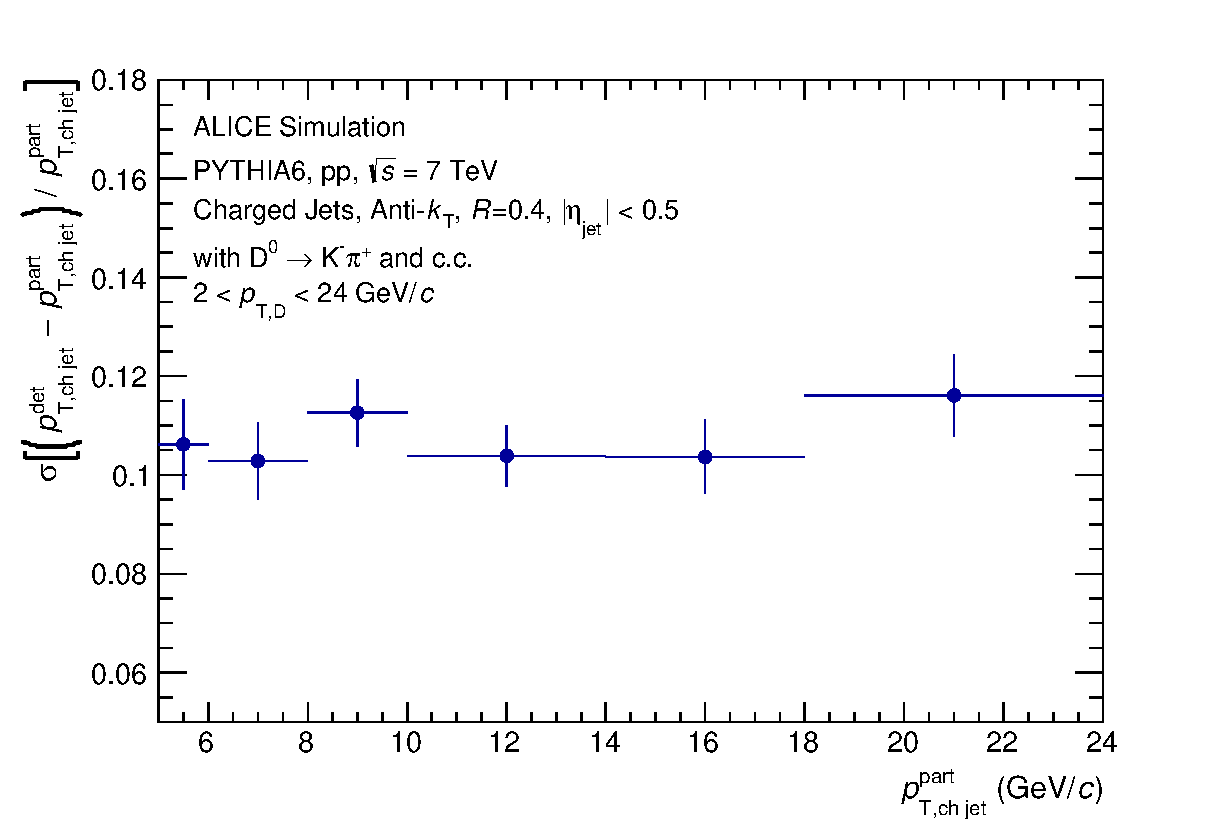
\includegraphics[width=.36\textwidth]{img/HQ16_Simulation_Resolution}

No significant \pt-dependence of the JES shift and resolution in the range $5<\ptchjet<24$~\GeVc
\end{frame}

\section{Signal Extraction}

\subsection{D-tagged jet signal extraction}

\begin{frame}{Signal extraction: invariant mass fit}
\begin{columns}

\column{.5\textwidth}
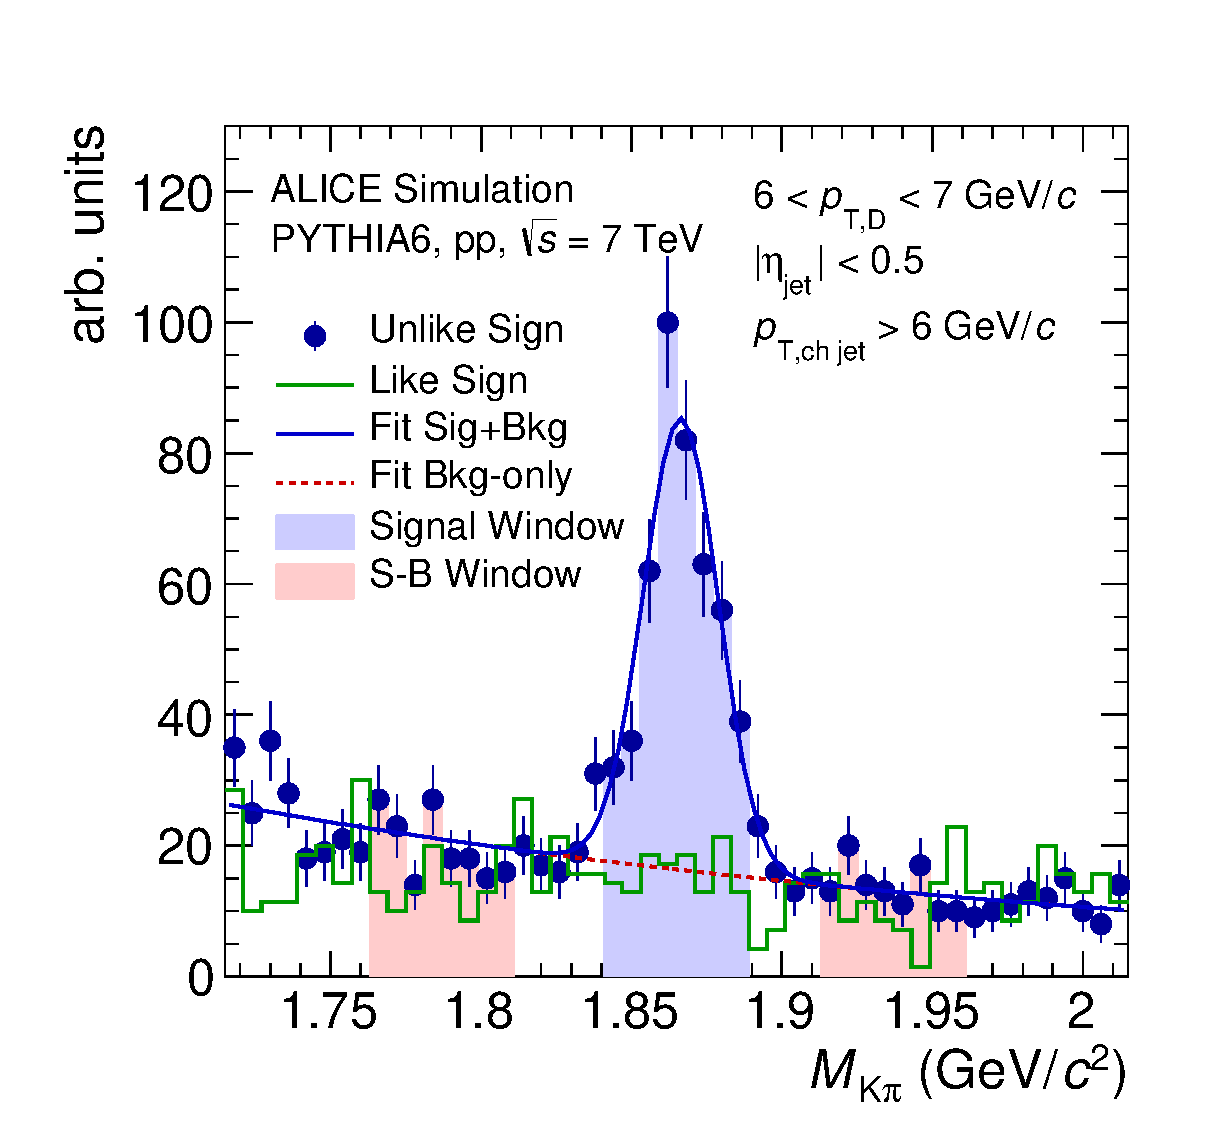
\includegraphics[width=\textwidth]{img/HQ16_Simulation_InvMassSB}

\column{.5\textwidth}
\textbf{\alert{Method 1: invariant mass fit}}
\begin{enumerate}
\item Bin D-tagged jet candidates in \alert{\ptchjet}
\item \alert{Fit invariant mass distributions} with a Gaussian (signal) + exponential (background)
\item Extract signal from fit parameters
\end{enumerate}
\end{columns}
\begin{itemize}
\item The correction for the D-tagged jet reconstruction efficiency must be applied as a weight when filling the invariant mass plots
\end{itemize}
\end{frame}

\begin{frame}{Signal extraction: SB and LS methods}
\begin{columns}

\column{.5\textwidth}
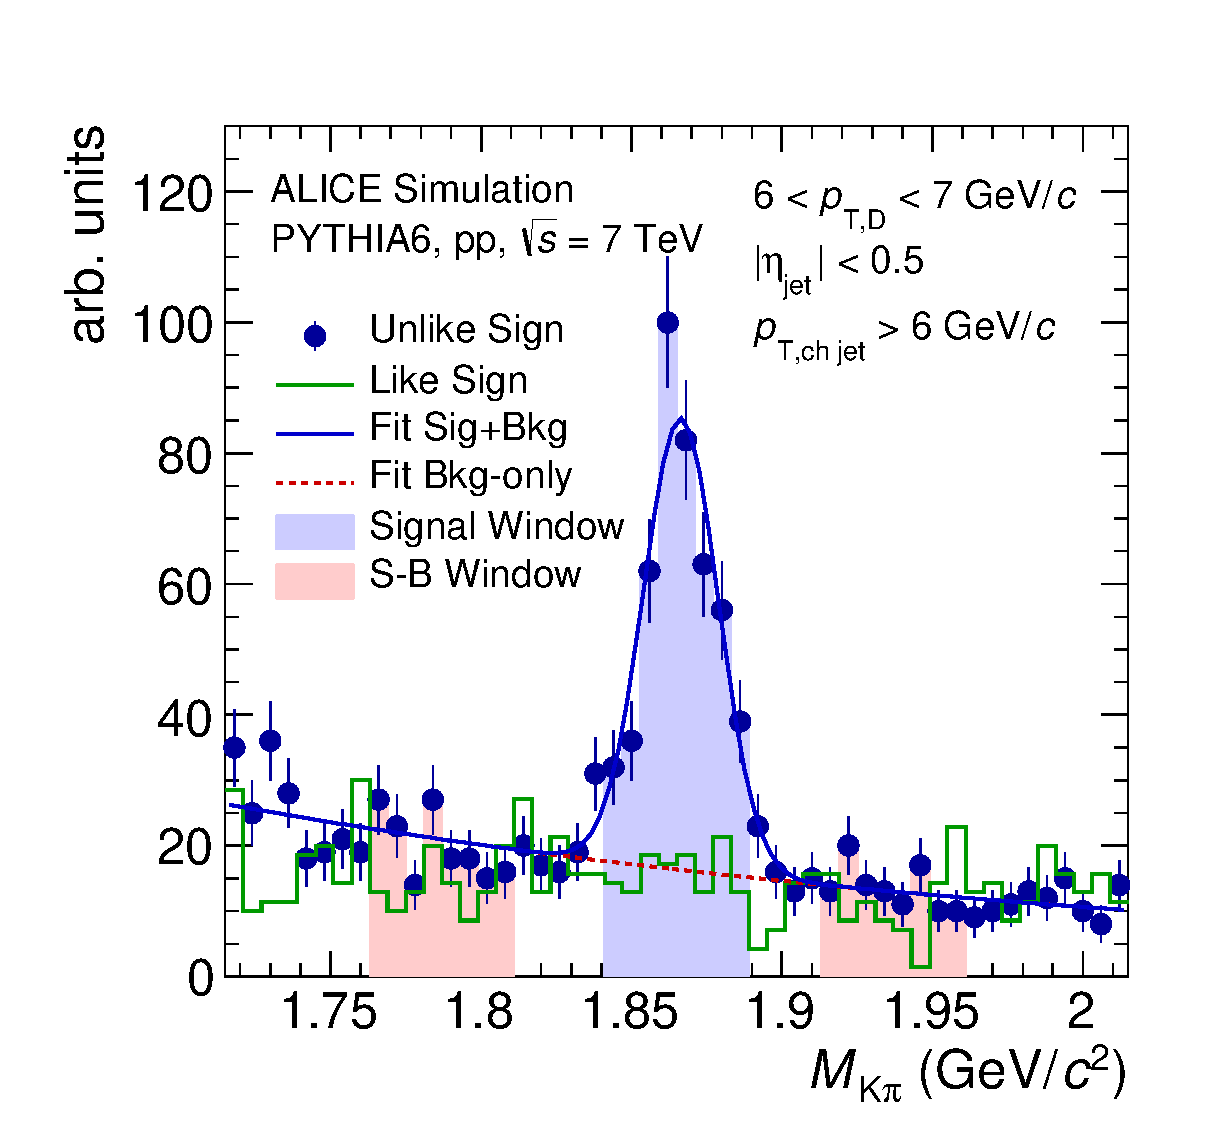
\includegraphics[width=\textwidth]{img/HQ16_Simulation_InvMassSB}

\column{.5\textwidth}
\textbf{\alert{Method 2: Side-Bands (SB) or Like-Sign (LS)}}
\begin{enumerate}
\item Bin D-tagged jet candidates in \ptd
\item Extract signal
\end{enumerate}

\textcolor{blue}{In the peak area: $|M_{\rm K\pi} - M_{\rm fit}| <2\sigma$\\ $N_{\rm sig+bkg} (\ptchjet, \ptd)$}

\textcolor{red}{In the SB: $8\sigma <|M_{\rm K\pi} - M_{\rm fit}| < 4\sigma$\\ $N_{\rm bkg, SB} (\ptchjet, \ptd)$}

\textcolor{green}{In the peak area for LS \\ $N_{\rm bkg, LS} (\ptchjet, \ptd)$}

\end{columns}
\begin{enumerate}
\setcounter{enumi}{2}
\item Apply efficiency correction and integrate in \ptd
$$N_{\rm signal} (\ptjet)=\sum_{\ptd} \frac{1}{\epsilon(\ptd)} [N_{\rm sig+bkg}(\ptjet, \ptd) - N_{\rm bkg}(\ptjet, \ptd)]$$
\end{enumerate}
\end{frame}

\subsection{Method comparison}
\begin{frame}{Method comparison}
\begin{columns}
\column{.6\textwidth}
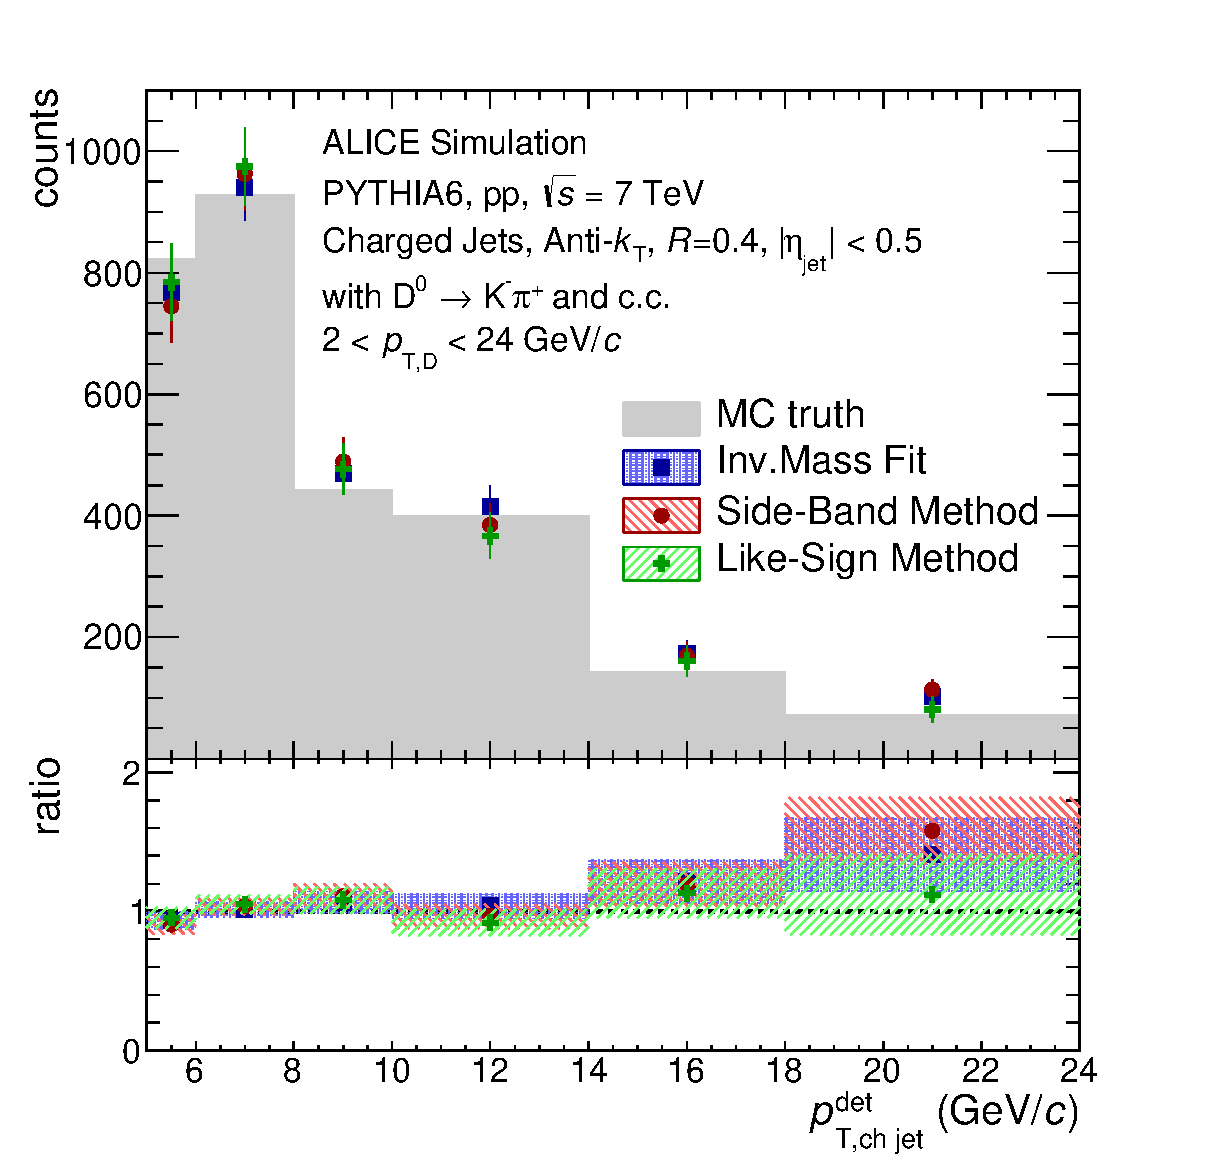
\includegraphics[width=\textwidth]{img/HQ16_Simulation_MethodComparison}
\column{.4\textwidth}
\begin{itemize}
\item D-tagged jet signal yields extracted using the  \textcolor{blue}{invariant mass fit}, \textcolor{red}{Side-Band} and  \textcolor{green}{Like-Sign} methods are compared with the  \textcolor{gray}{MC truth}
\item All methods \textbf{agree well} with the MC truth within their statistical uncertainty
\end{itemize}
\end{columns}
\end{frame}

\subsection{Statistical precision}
\begin{frame}{Statistical precision}
\begin{columns}
\column{.6\textwidth}
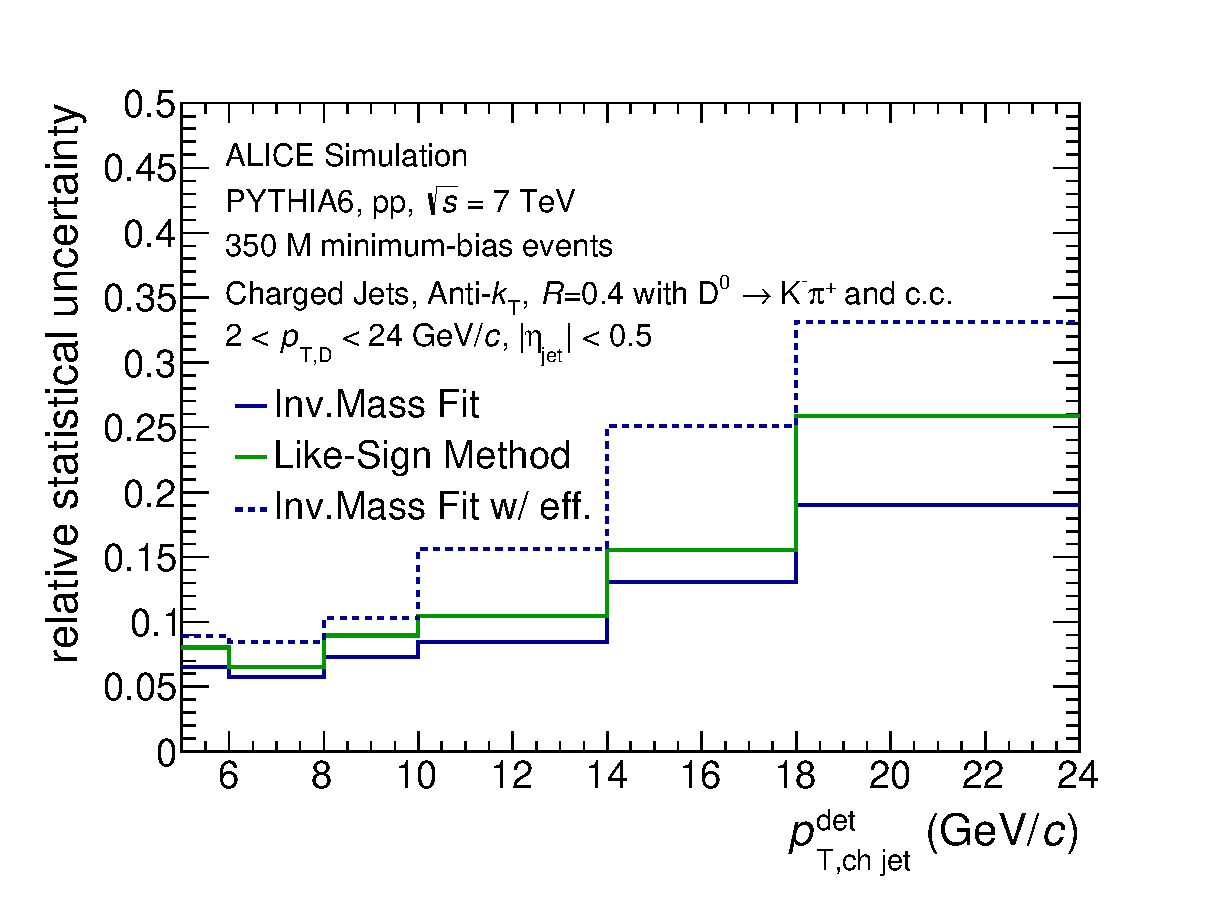
\includegraphics[width=\textwidth]{img/HQ16_Simulation_UncertaintyComparison}

\column{.4\textwidth}
\begin{itemize}
\item The methods differ also for their \alert{statistical precision}
\item[$\rightarrow$] larger uncertainties for LS method
\item The \alert{efficiency correction} alters the relative contribution of D-mesons with different \pt
\item[$\rightarrow$] the relative statistical uncertainty increases
\end{itemize}
\end{columns}
\end{frame}

\section*{Summary}

\subsection*{Conclusions}
\begin{frame}{Conclusions}
\begin{itemize}
\item The measurement of the charm cross-section and fragmentation function provides a important tools for
testing pQCD and probing the QGP
\item 3 different techniques have been developed to extract the D-tagged jet yield:
\begin{itemize}
\item Invariant mass fit in bins of \ptjet
\item Bin counting in the peak area w/ Like-Sign background subtraction
\item Bin counting in the peak area w/ Side-Band background subtraction
\end{itemize}
\item Proved to be feasible and successfully tested in Monte Carlo
\item The pros and cons of each technique is being assessed
\item Now looking forward to finalize the analysis on real data!
\end{itemize}
\end{frame}

\subsection*{Stay Tuned: Work In Progress!}
\begin{frame}{Stay Tuned: Work In Progress!}
\begin{columns}
\column{.55\textwidth}
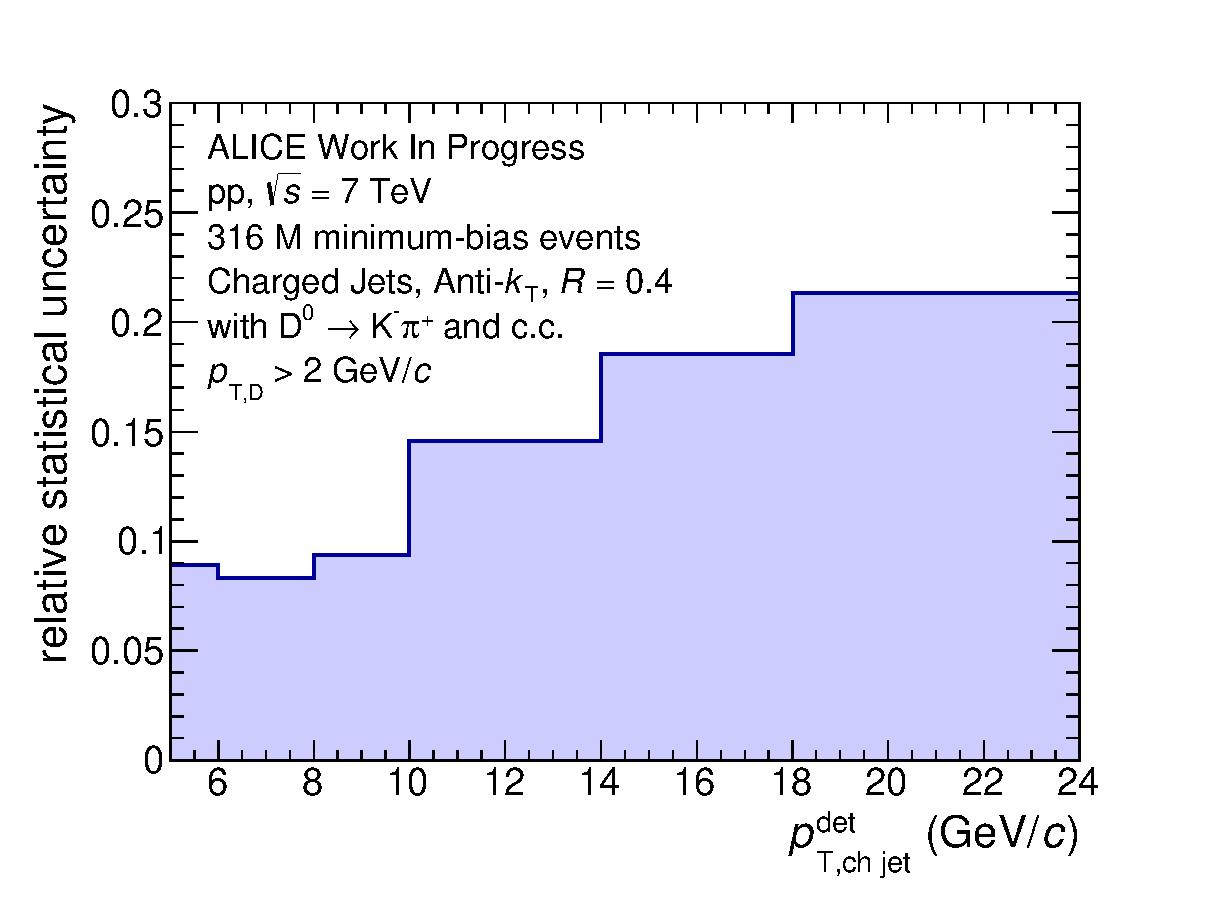
\includegraphics[width=\textwidth]{img/HQ16_WorkInProgress_StatisticalUncertainty}
\column{.45\textwidth}
\begin{itemize}
\item The analysis is being performed using data collected by ALICE with pp collisions at 7 TeV
\item A preliminary look at the available statistics in 2010 data has given promising expectation
\item Look out for new results being made public soon!
\end{itemize}
\end{columns}
\end{frame}

% All of the following is optional and typically not needed. 
%\appendix
%\section<presentation>*{\appendixname}
%\subsection<presentation>*{Backup}

%\begin{frame}
 % \frametitle<presentation>{Backup 1}    
%\end{frame}

\end{document}
